\documentclass[twocolumn,superscriptaddress,aps]{revtex4-1}

\usepackage[utf8]{inputenc}

\usepackage{amsfonts}
\usepackage{amssymb}
\usepackage{amsmath}
\usepackage{amsthm}

\usepackage{bbold}
\usepackage{bm}
\usepackage{color}
\usepackage{hyperref}
\usepackage{graphicx}
\graphicspath{{figures/}}

\begin{document}


% ==============================================================================

\title{\Large{INFO8010: Brain Cancer Detection Project Report}}
\vspace{1cm}
\author{\small{\bf Ayoub Assaoud}}
\affiliation{\texttt{ayoub.assaoud@student.uliege.be} (\texttt{s207227})}

\maketitle
\section{Abstract}

\section{Introduction}
%%% Introduction: which states the problem which has been tackled

For this project we propose to build a generative deep learning system that can generate anime faces. The system will be trained on a dataset of anime faces and will use denoising diffusion probabilistic models (DDPM) to generate new faces. The goal is to create a system that can generate acceptable quality anime faces that are diverse and realistic by drawing samples, and naturally for denoising by encoding-decoding the image. The project will also explore the use of different architectures and techniques to improve the quality of the generated faces.

Through this project, we:

\begin{itemize}
        \item Collecte and preprocess over than 80,000 anime face images, applying normalization, resizing, and few augmentations.
        \item Design and train two distinct deep learning models, mainly noise prediction technique and have a quick view on score-based energy model, experimenting with different architectures and training strategies.
        \item Evaluate performance using some basic metrics.
    \end{itemize}

In the following sections, we'll walk through related work, our data pipeline, model Architecture, and results.

\section{Related Work}
%%% Related Work: which covers research that is related to the considered problem


\section{Methods}
%%% Methods: a clear and detailed description of the neural networks (architecture, training-parameters, loss function, data)
\subsection{Data}
\subsubsection{Dataset Description}

%TODO: some image samples
% \begin{figure}[htbp]
%     \centering
%     \includegraphics[width=0.5\textwidth]{figures/dataset_sample.png}
%     \caption{A sample of MRI images from the brain tumor dataset.}
%     \label{Figure 1: dataset}
% \end{figure}

\subsubsection{Data Preprocessing}
Our preprocessing pipeline was implemented in Python using PyTorch library, and included the following steps:

\begin{itemize}
    \item \textbf{Normalization:} We normalize the pixel values to the range [-1, 1], to keep consistent with the noise distribution. an it seems to be much more effective than constraining the model to output values in the required range.
    \item \textbf{Resizing:} All images were resized to a fixed size of 64x64 pixels.
    \item \textbf{Data Augmentation:} We applied random horizontal flipping to increase dataset diversity, no rotation or cropping was applied because most faces were not centered, or touching the frame, which could lead to poor generated samples.
\end{itemize}

%%%%%%%%%%%%%%%%%%%%%%%%%%%%%%%%%%%%%%%%%%%%%%%%%%%%%%%%%%%%%%%%%%%%%%%%%%%%%%%%%%%%%%%
\subsection{Architecture}
We use a denoising diffusion probabilistic model (DDPM) as the backbone of our generative system. The DDPM consists of a forward diffusion process that gradually adds gaussian noise to the data, and a reverse diffusion process that learns to denoise the data. This architecture allows for high-quality image generation by sampling from the learned distribution.

the same architecture can be used to approximate the score function of the data distribution $s_\theta(x , t) \approx \nabla \log p_t(x_t)$.

\subsubsection{Description}

We explore several variants of the DDPM architecture, including:

\begin{itemize}
    \item \textbf{U-Net Backbone:} A U-Net architecture is used as the denoiser model that predicts the original noise $\epsilon \approx\epsilon_\theta(x_t, t)$ for the DDPM.
    \item \textbf{ResNet Blocks:} We incorporate residual blocks to improve the flow of gradients during training, which helps in learning complex features.
    \item \textbf{Attention Mechanisms:} We incorporate attention mechanisms to improve the model's ability to focus on relevant features during the denoising process.
\end{itemize}

The Unet architecture consists of Three main components: a chain of $down_channels$ \textbf{DownEncoder}, a chain of $mid_channels$ \textbf{Bottleneck}, and a chain of $down_channels$ \textbf{UpDecoder}, to preserve symmetric feature mapping.

The DownEncoder reduces the spatial dimensions of the input image while increasing the number of feature channels, allowing the model to learn hierarchical representations.

The Bottleneck connects the DownEncoder and UpDecoder, serving as a bridge that captures the most abstract features.

The UpDecoder then reconstructs the image by progressively increasing the spatial dimensions while reducing the number of feature channels (Up sampling).

Each of these subcomponents is composed of $\#ModelParams.num_(down\|mid\|up)_layers$ \textbf{block layers}, each of these block layers consists of a stack of $\#ModelParams.num_(down\|mid\|up)_layers$ ResNet block followed by a self-attention layer (optionnel in our case see discussion) and finally an optionnel convolutive layer (downsampling or upsampling), see figure bellow.

\begin{figure*}[ht]
  \centering
  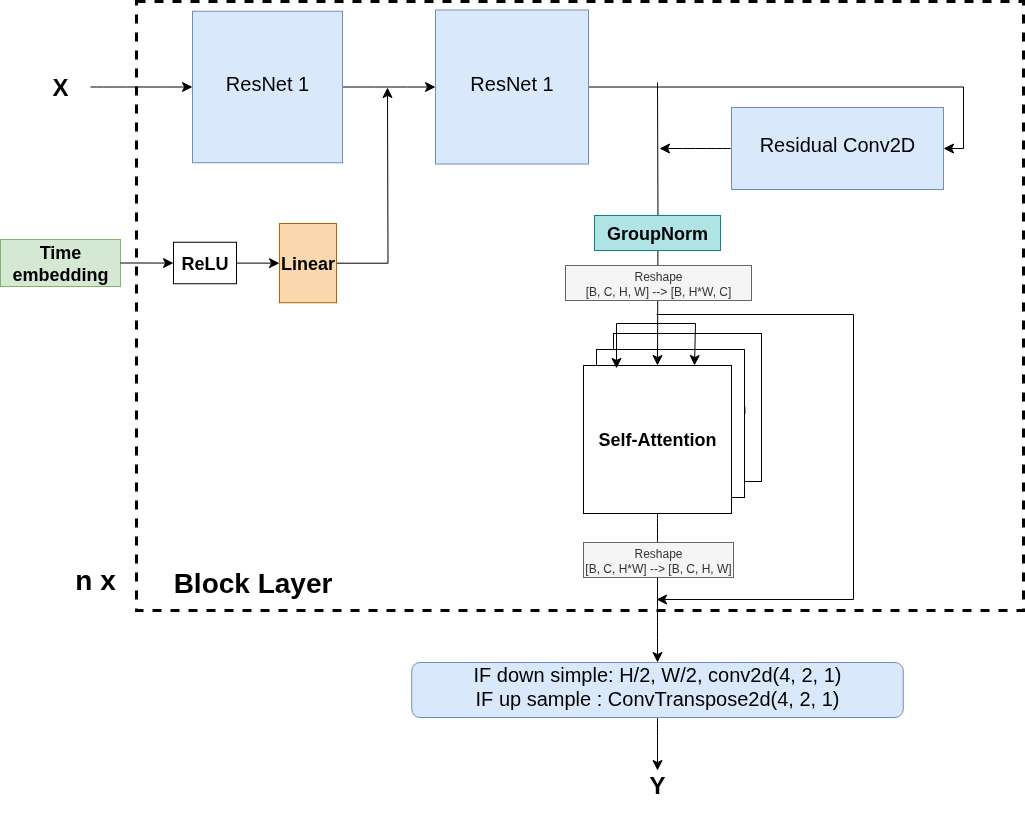
\includegraphics[width=\textwidth]{figures/block_layer.png}
  \caption{Block layer Architecture with ResNet blocks and self-attention layers.}
  \label{fig:unet_architecture}
\end{figure*}

The ResNet block consists of two convolutional layers with Group normalization and SiLU activation, allowing the model to learn residual mappings, and the input is added to a \textbf{positional embedding learnable vector} after the first convolutional layer, whereas the self-attention layer allows the model to focus on relevant features in the input image, improving the quality of the generated images.

The DownEncoder uses strided convolutions to reduce the spatial dimensions, while the UpDecoder uses transposed convolutions to increase them. The Bottleneck uses standard convolutions without striding.


% %%%%%%%%%%%%%%%%%%%%%%%%%%%%%%%%%%%%%%%%%%%%%%%%%%%%%%%%%%%%%%%%%%%%%%%%%%%%%%%%%%%%%%%
\subsubsection{Motivating choices}

\textbf{the choice of activation function:} we choosed SiLU (Sigmoid Linear Unit) as the activation function for the model, which is known to improve the flow of gradients and enhance the model's ability to learn complex features. SiLU has been shown to outperform ReLU in many cases, especially in image-tasks.
in other point of view, image pixels are normalized to the range [-1, 1], and the SiLU activation function is well-suited for this range, as it smoothly transitions between negative and positive values.

\textbf{the choice of normalization:} we used Group Normalization instead of Batch Normalization, to normalize the features within groups, which is more effective in stabilizing training, especially that in our cases where batch size is set to 6 which is small because of reaching GPU Limit, it is also good for variable batch size while evaluation.

\textbf{the choice of attention mechanism:} as modern architectures often incorporate attention mechanisms, we used self-attention layers to allow the model to focus on relevant features in the input image, improving the quality of the generated images. Self-attention helps the model capture long-range dependencies and relationships between pixels, which is crucial for generating high-quality images.

this desicion has an impact, as we will soonly see, that there is a trade-off between an attention block for each block layer and the model's performance, as it increases the number of parameters, requires more data to train, sensible to noise, and increases the training time. 

we will get a tour over the architecture we have tried in the order time we 
% In our case, we found that using attention in the first two block layers of the DownEncoder and UpDecoder was sufficient to achieve good results without significantly increasing the model's complexity. 


% %%%%%%%%%%%%%%%%%%%%%%%%%%%%%%%%%%%%%%%%%%%%%%%%%%%%%%%%%%%%%%%%%%%%%%%%%%%%%%%%%%%%%%%

% as we progress through epochs, small models tend to overfit very fast, 10M and 49M reaches their best generation respectively 1 and 3 but still very low quality, then they tend to denoise images but very low generation quality, while larger models 74M and 85M tend to perform poorly in earlest epochs, and then  generate better quality images respectivly 7 and %TODO but require more data to train and are more sensitive to noise in later time steps.

% we choosed to not consider the upsamplinf factor in the MSE $\frac{1}{2\sigma_t^2} \frac{(1 - \sigma_t)^2}{(1 - \hat \sigma_t) \sigma_t}$


\subsubsection{Mini U-Net DDPM Architecture: 10M}


% %%%%%%%%%%%%%%%%%%%%%%%%%%%%%%%%%%%%%%%%%%%%%%%%%%%%%%%%%%%%%%%%%%%%%%%%%%%%%%%%%%%%%%%

% \subsection{Training}
% \subsubsection{Parameters}


% \subsubsection{Training Procedure}

% \subsubsection{Optimizer}
% We used the AdamW optimizer, which is an extension of the Adam optimizer with weight decay. AdamW helps to prevent overfitting by adding a weight decay term to the loss function, which encourages the model to learn simpler representations.

% the desicion to use AdamW was based on its effectiveness in training deep learning models, especially in the context of image classification tasks. It combines the benefits of adaptive learning rates and weight decay.

% we kept the default parameters for AdamW, which are:
% \begin{table}[h]
%     \centering
%     \begin{tabular}{|c|c|c|c|c|}
%         \hline
%         $\beta_1$ & $\beta_2$ & $\epsilon$ & weight decay & learning rate \\
%         \hline
%         0.9 & 0.999 & 1e-8 & 1e-4 & 1e-4 \\
%         \hline
%     \end{tabular}
%     \caption{Optimizer Parameters}
%     \label{tab:optimizer_params}
% \end{table}

% \subsubsection{Loss Function}
% the loss function used for training the models is the Cross-Entropy loss, which is commonly used for multi-class classification tasks. It measures the dissimilarity between the predicted class probabilities and the true class labels.
% The Cross-Entropy loss is defined as:
% \[
% L = - \sum_{i=1}^{N} \sum_{j=1}^{3} y_{i,j} \log(p_{i,j})
% \]
% $y_{i,j}$ is 1 if sample i belongs to class j, otherwise 0\\
% $p_{i,j}$ is the predicted probability for class j.

% thus even if the model predicts a probability of 0.8 for the correct class and 0.2 for the other classes, it will be penalized for this low confidence, but the loss will be low accordingly.


% \section{Results}

% \begin{figure*}[ht]
%   \centering
%   \includegraphics[width=\textwidth]{figures/train-and-test-accuracies-averaged2.png}
%   \caption{Evolution of Training and validation accuracies for each model.}
%   \label{fig:train-val-acc}
% \end{figure*}

% % \begin{figure*}[ht]
% %   \centering
% %   \includegraphics[width=\textwidth]{figures/train-and-test-losses-averaged.png}
% %   \caption{Evolution of Training and validation losses for each model.}
% %   \label{fig:train-val-loss}
% % \end{figure*}


\section{Discussion} %and future improvements

\subsection{The}

\subsection{The importance of }


\subsection{The importance of }


\subsection{The importance of cropping images}

\subsection{About possible improvements}

% ==============================================================================
\newpage
\section{References}

\bibliographystyle{IEEEtran}
\bibliography{bibiography}

\end{document}